\chapter{analysis}

\section{Background}
	Aggregation tree
	Commitment tree
	Analogy with binary representation
\section{Star Tree}
	
	To do : Material on star tree, star tree analysis gives you 1 cert savings.

	\begin{figure}[H]\label{star-aggregation-tree}
  	\centering
  		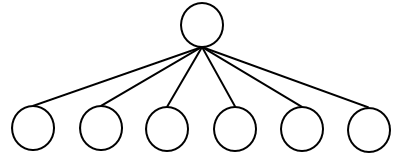
\includegraphics[scale=0.4]{images/star-tree.png}\\
  		\caption{Star aggregation tree}
  \end{figure}

\newpage

\section{Maximum savings}
	Analysis is true for any n bit forest size.	Give names to the following tolopogies.  
	\textbf{Maximum savings}, with n(=4) bit forest, fanout(=2), savings of n(=4) certificates:

	\begin{figure}[hp]
		\centering
		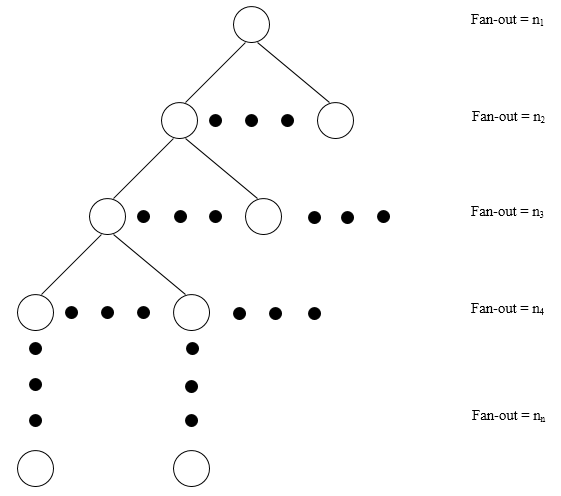
\includegraphics[scale=0.5]{images/symmetric-tree.png}\\
		\caption{Symmetric Tree}
	\end{figure}

	\begin{multicols}{2}

		\begin{tabular}{ l | l l c r }
		  1 & 1 & 1 & 1 & 0 \\
		  \hline
		  0 & 1 & 1 & 1 & 1 \\
		  0 & 1 & 1 & 1 & 1 \\
		  0 & 0 & 0 & 0 & 1 \\
		  \hline	
		  A & C & C & C & C\\
		\end{tabular}
	\columnbreak{|}
		\begin{tabular}{ l | l l c r }
		  1 & 1 & 1 & 1 & 0 \\
		  \hline
		  0 & 1 & 1 & 1 & 1 \\
		  0 & 1 & 1 & 1 & 1 \\
		  0 & 0 & 0 & 0 & 1 \\
		  \hline	
		  A & A & A & A & A\\
		\end{tabular}
	\end{multicols}

	\textbf{No savings}, with n(=4) bit forest with alternate bit positions, fanout(=2, 3, 5) :

	\begin{multicols}{3}

		\begin{tabular}{ l |l l c r }
		  
		  1 & 0 & 1 & 0 & 0 \\
		  \hline
		  0 & 1 & 0 & 1 & 0 \\
		  0 & 1 & 0 & 1 & 0 \\
		  0 & 0 & 0 & 0 & 1 \\
		  \hline	
		  A & 0 & A & 0 & A \\
		
		\end{tabular}
		\columnbreak{|}
		\begin{tabular}{ l |l l c r }
		  
		  1 & 0 & 1 & 0 & 0 \\
		  \hline
		  0 & 1 & 0 & 1 & 0 \\
		  0 & 1 & 0 & 1 & 0 \\
		  0 & 1 & 0 & 1 & 0 \\
		  0 & 0 & 0 & 0 & 1 \\
		  \hline	
		  A & C & A & C & A \\
		
		\end{tabular}
		\columnbreak{|}
		\begin{tabular}{ l l |l l c r }
		  
		  0 & 1 & 0 & 0 & 0 & 0 \\
		  0 & 1 & 0 & 1 & 0 & 0 \\
		  1 & 1 & 1 & 1 & 0 & 0 \\
		  \hline
		  0 & 0 & 1 & 0 & 1 & 0 \\
		  0 & 0 & 1 & 0 & 1 & 0 \\
		  0 & 0 & 1 & 0 & 1 & 0 \\
		  0 & 0 & 1 & 0 & 1 & 0 \\
		  0 & 0 & 1 & 0 & 1 & 0 \\
		  0 & 0 & 0 & 0 & 0 & 1 \\
		  \hline	
		  A & A & 0 & 0 & C & A \\
		
		\end{tabular}

	\end{multicols}

	\newpage

	 \textbf{Savings of n - 1 certificates}, with n(=4) bit forest, fanout(=3) :

	\begin{multicols}{2}

		\begin{tabular}{ l l |l l c r }
		  0 & 1 & 1 & 1 & 1 & 0 \\
		  1 & 1 & 1 & 1 & 1 & 0 \\
		  \hline
		  0 & 0 & 1 & 1 & 1 & 1 \\
		  0 & 0 & 1 & 1 & 1 & 1 \\
		  0 & 0 & 1 & 1 & 1 & 1 \\
		  0 & 0 & 0 & 0 & 0 & 1 \\
		  \hline	
		  A & 0 & C & C & C & 0 \\
		\end{tabular}
	\columnbreak{|}
		\begin{tabular}{ l l | l l c r }
		  0 & 1 & 1 & 1 & 1 & 0 \\
		  1 & 1 & 1 & 1 & 1 & 0 \\
		  \hline
		  0 & 0 & 1 & 1 & 1 & 1 \\
		  0 & 0 & 1 & 1 & 1 & 1 \\
		  0 & 0 & 1 & 1 & 1 & 1 \\
		  0 & 0 & 0 & 0 & 0 & 1 \\
		  \hline
		  A & 0 & A & A & A & 0\\

		\end{tabular}

	\end{multicols}

	\textbf{Savings of n - 1 certificates}, with n(=4) bit forest, fanout(=4) :

	\begin{multicols}{2}

		\begin{tabular}{ l l |l l c r }
		  
		  0 & 1 & 1 & 1 & 0 & 0 \\
		  0 & 1 & 1 & 1 & 1 & 0 \\
		  1 & 1 & 1 & 1 & 1 & 0 \\
		  \hline
		  0 & 0 & 1 & 1 & 1 & 1 \\
		  0 & 0 & 1 & 1 & 1 & 1 \\
		  0 & 0 & 1 & 1 & 1 & 1 \\
		  0 & 0 & 1 & 1 & 1 & 1 \\
		  0 & 0 & 0 & 0 & 0 & 1 \\
		  \hline	
		  A & A & C & C & 0 & C \\
		
		\end{tabular}
	\columnbreak{|}
		\begin{tabular}{ l l | l l c r }
		  0 & 1 & 1 & 1 & 0 & 0 \\
		  0 & 1 & 1 & 1 & 1 & 0 \\
		  1 & 1 & 1 & 1 & 1 & 0 \\
		  \hline
		  0 & 0 & 1 & 1 & 1 & 1 \\
		  0 & 0 & 1 & 1 & 1 & 1 \\
		  0 & 0 & 1 & 1 & 1 & 1 \\
		  0 & 0 & 1 & 1 & 1 & 1 \\
		  0 & 0 & 0 & 0 & 0 & 1 \\
		  \hline
		  A & A & A & A & 0 & A\\

		\end{tabular}

	\end{multicols}

\newpage

\section{Pseudo Palm Tree}
	
	\begin{figure}[hp]
		\centering
		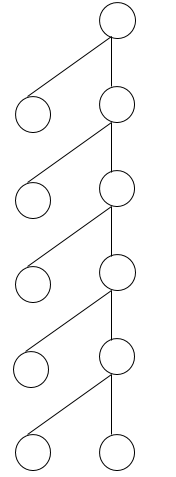
\includegraphics[scale = 0.3]{images/pseudo-palm-tree}
		\caption{Pseudo palm tree}
		\label{fig:pseudo}
	\end{figure}

	\begin{theorem}
		At any given level, if an aggregator priorities aggregating its childrens' messages over its own message, it can save bandwidth by not sending its childrens' certificates to its parent.
	\end{theorem}

	\begin{proof}
		We can see from Figure~\ref{fig:pseudo} that every aggregator has odd number of messages to aggregate, including itself.
		It means an aggregator at each level has odd number of $1's$ in therir least significant bits. 
		If an aggregator aggregates messages of its children and creates a carry then it needs to send its own certificate to its parent or else it has to send one of its children's certificate as well.
		Following example illustrates the idea, where C means an aggregator has to send its child's certificate to its parent, A means an aggregator has to send its own certificate to its parent and X is don't care.
		\begin{multicols}{2}
			\begin{tabular}{ l | l l l l }
				0 & 0 & 0 & 1 & 0 \\
				\hline
				0 & 0 & 0 & 0 & 1 \\
				0 & 0 & 0 & 0 & 1 \\
				X & X & X & X & 1 \\
				\hline
				X & X & X & X & C \\
			\end{tabular}
			\columnbreak{|}
			\begin{tabular}{ l | l l l l }
				0 & 0 & 0 & 1 & 0 \\
				\hline
				0 & 0 & 0 & 0 & 1 \\
				0 & 0 & 0 & 0 & 1 \\
				X & X & X & X & 1 \\
				\hline
				X & X & X & X & A \\
			\end{tabular}
		\end{multicols}
		
		Hence, this approach saves bandwidth by sending one less certificate at each level. 
	
	\end{proof}

\section{Binary tree}
	\begin{figure}[hp]
		\centering
		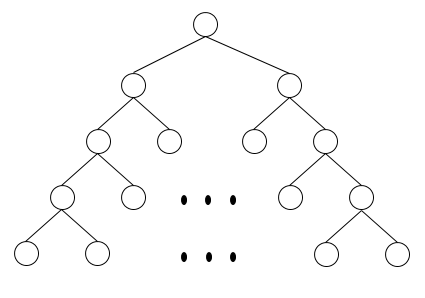
\includegraphics[scale = 0.3]{images/binary-tree}
		\caption{Binary tree}
		\label{fig:binary}
	\end{figure}

	\begin{theorem}
		At any given level, if an aggregator priorities aggregating its childrens' messages over its own message, it can save bandwidth by not sending $\lceil lg(n /2) \rceil$ certificates, n is number of descendants for given node, to its parent.
	\end{theorem}